\documentclass{article}

\usepackage{corl_2026}
\usepackage{booktabs}
\usepackage{graphicx}
\usepackage{microtype}
\usepackage{xspace}

\title{Containment Without Competence: Evaluating Validation Pipelines for Language-Based Multi-UAV Planning}

\author{Anonymous Authors}

\newcommand{\Mone}{\textsc{M1}\xspace}
\newcommand{\Mtwo}{\textsc{M2}\xspace}
\newcommand{\Mthree}{\textsc{M3}\xspace}
\newcommand{\Mfour}{\textsc{M4}\xspace}

\begin{document}
\maketitle

\begin{abstract}
Language-based robot planners can produce fluent plans despite missing evidence
or conflicting resources. We compare four validation-pipeline configurations
on 1,420 controlled derivatives of 284 held-out MultiUAV-Plat tasks using frozen
Qwen2.5-3B and 7B checkpoints. Stage-wise validation eliminated unsupported
continuation on all 568 non-executable cases, but failed every one of 852
executable cases. A zero-call policy that always blocks achieved 20.0\% strict
success, exceeding the 7B stage-wise configuration's 16.1\%, showing that
containment alone does not establish useful discrimination. A post-hoc audit
also found that the frozen validator rejected 43 of 249 fully instantiated
upstream reference plans. The study is therefore a negative evaluation result:
pipeline configuration changes where failures stop, but the tested system does
not demonstrate executable planning or a causal effect of validation placement.
\end{abstract}

\keywords{physical AI safety, robot planning, failure containment, evaluation}

\section{Introduction}

An open-ended language interface can hide a consequential physical-AI failure:
a response may appear executable while relying on evidence that is absent from
the robot's visible context. Prior systems combine language models with
supervision, structured planning, and motion constraints
\citep{tacos,roco,llamar,commandswarm}. These systems motivate modular safety
checks, but they do not resolve how to evaluate a planner that avoids unsafe
continuation by refusing useful requests.

We study this distinction using controlled MultiUAV-Plat derivatives
\citep{multiuav_plat}. Here, \emph{containment} means that a pipeline does not
advance on a registered non-executable case. \emph{Static plan fidelity} means
conformance with frozen schema, endpoint, parameter, and command validators; it
does not mean simulator or physical success. Our contributions are: (1) a
paired five-variant benchmark for evidence availability and resource conflict;
(2) a comparison of four complete validation pipelines with frozen model and
prompt versions; and (3) a refusal-aware analysis that separates containment
from executable competence and audits the validator against upstream plans.

\section{Experimental Design}

\paragraph{Cases.}
The pinned source contains 1,500 tasks in 75 sessions. Deterministic duplicate
and leakage checks retained 1,473 source tasks, split by session into 899 train,
290 calibration, and 284 test clusters. Each held-out cluster yields five linked
cases: canonical execute, official-alias execute, missing-evidence clarify,
restored-evidence execute, and resource-conflict block. The test matrix contains
1,420 cases per method and model: 852 executable and 568 non-executable. A
stratified 30-cluster pilot checked construction quality; it was not a complete
human audit.

\paragraph{Configurations.}
\Mone is a one-call monolithic planner. \Mtwo adds a deterministic post-plan
gate. \Mthree builds and checks an evidence ledger before planning and validates
provenance afterward. \Mfour is a two-call post-plan configuration that is
\emph{model-call-count-matched} to \Mthree. The comparison does not isolate
placement: \Mthree and \Mfour also differ in prompts, validation behavior,
generated content, and token counts. We therefore compare complete pipeline
configurations rather than claim a causal placement effect.

\paragraph{Models and outcomes.}
We use immutable Qwen2.5-3B-Instruct and Qwen2.5-7B-Instruct revisions with
deterministic decoding. Registered outcomes are unsupported continuation on
the 568 non-executable cases and strict success over all 1,420 cases. Executable
success requires the correct disposition and a non-empty plan passing every
static validator; non-executable success requires the exact clarify or block
disposition without a prohibited plan. Registered paired differences are
aggregated by source task and use 10,000 fixed-seed percentile-bootstrap draws.

\paragraph{Post-hoc reviewer diagnostics.}
We score a deterministic always-\textsc{Block} reference over unique cases,
repeat paired contrasts by resampling the 15 held-out sessions, partition every
executable failure into one observed location, and pass fully instantiated
upstream API plans through the frozen validator. Unresolved upstream templates
are excluded rather than imputed. These diagnostics do not change the
registered analysis and invoke no model.

\section{Results}

Figure~\ref{fig:outcomes} separates two positively oriented outcomes. For 3B,
containment rates for \Mone--\Mfour were 21.0\%, 99.6\%, 100\%, and 99.8\%; all
strict-success rates were zero. For 7B, containment was 31.7\%, 97.7\%, 100\%,
and 97.4\%, while strict success was 0\%, 0\%, 16.1\%, and 0.8\%. Every nonzero
strict success was a correct non-executable outcome. All eight model--method
conditions had 0/852 executable static plan fidelity.

\begin{figure}[t]
  \centering
  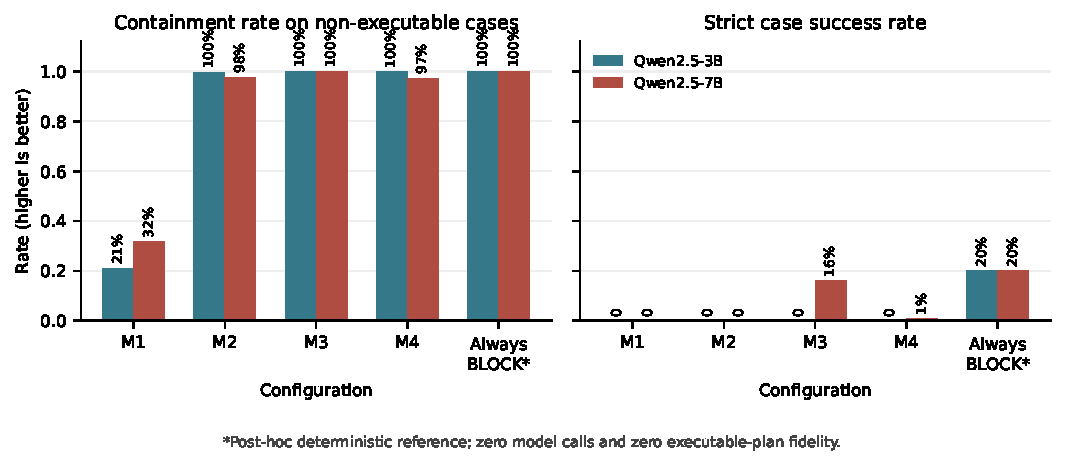
\includegraphics[width=\linewidth]{accuracy_refusal_aware_outcomes_v2.pdf}
  \caption{Containment and strict success, both higher-is-better. Always-
  \textsc{Block} is a post-hoc zero-call reference with zero executable-plan
  fidelity.}
  \label{fig:outcomes}
\end{figure}

Always-\textsc{Block} contained every non-executable case and correctly handled
the 284 conflict cases, producing 284/1,420 (20.0\%) strict success. It exceeded
7B \Mthree's 228/1,420 (16.1\%) while falsely blocking all 852 executable and
all 284 clarification cases. Thus, perfect containment and the aggregate
strict-success metric do not demonstrate useful discrimination.

The registered 7B \Mthree{} minus \Mone differences were $-0.6831$ for
unsupported continuation (95\% interval $[-0.7324,-0.6338]$) and $0.1606$ for
strict success ($[0.1507,0.1697]$). Session-clustered sensitivity preserved the
directions: $-0.6829$ ($[-0.7220,-0.6373]$) and $0.1605$
($[0.1513,0.1688]$), respectively. Only 15 sessions were available, so this is
a robustness check rather than a rich hierarchical analysis.

\paragraph{Where executable cases failed.}
For 3B \Mthree, 544/852 executable cases stopped before planning and 308/852
failed output parsing. For 7B \Mthree, 637/852 produced a model non-execution
decision, 187/852 failed output parsing, and 28/852 stopped before planning.
These mutually exclusive counts show that zero unsupported continuation was
obtained through over-conservatism, not successful executable planning.

\paragraph{Validator audit.}
Of 284 upstream reference plans, 249 were fully instantiated and 35 contained
unresolved or missing template fields. The frozen validator accepted 206/249
(82.7\%) and rejected 43/249 (17.3\%): one at endpoint schema, three at
parameter grounding, and 39 at safety bounds. Validator mismatch therefore
contributes to the zero-fidelity result, although it does not explain every
model failure.

\paragraph{Compute.}
A separate exploratory campaign measured 30 clusters, all five variants, four
methods, two models, and three repetitions on one RTX 3090. Relative to \Mone,
\Mthree increased 3B duration by 8.86--9.49~s and board energy by
1,565--1,681~J, but reduced 7B duration by 6.23--6.82~s and board energy by
1,153--1,245~J. Relative to model-call-count-matched \Mfour, 7B \Mthree
generated 446.82 fewer output tokens and used 5,669--6,279~J less board energy.
These differences are confounded by termination behavior and generated length;
they are not evidence that stage-wise validation is intrinsically cheaper.

\section{Discussion and Limitations}

The central result is containment without competence. \Mthree suppresses
unsupported continuation, but an indiscriminate block policy is stronger on
the aggregate success metric and no tested method produces a valid executable
plan. The official-plan audit additionally shows that the evaluation mechanism
itself rejects a nontrivial fraction of upstream plans. A stronger follow-up
must first reconcile and re-audit validator rules, then hold prompts and rules
fixed while changing only placement, and finally test execution in an official
environment.

The study uses controlled derivatives rather than live operator missions, two
sizes from one model family, a 30-cluster human pilot, and one GPU for resource
measurement. It performs no official simulator or physical execution. The
source-task bootstrap is registered; the session bootstrap is post-hoc and has
only 15 units. The resource campaign has three repetitions, and board energy is
not whole-system or UAV energy. These limits prevent claims of general robot
safety, practical mission capability, or causal superiority of one validation
placement.

\section{Conclusion}

Validation pipelines can move where failures are contained, but containment is
not evidence of planning competence. In this controlled study, stage-wise
validation eliminated unsupported continuation while failing every executable
case, underperforming always-\textsc{Block} on aggregate strict success, and
interacting with a validator that rejected 17.3\% of auditable upstream plans.
The defensible contribution is a refusal-aware evaluation protocol and a
negative empirical result that identifies what must be fixed before stronger
physical-AI safety claims are possible.

\bibliography{references}

\end{document}
